\chapter{Implementation}

In this chapter, we delve into the practical aspects of creating \gls{AI} agents capable of tackling abstract strategy games. The focus is on constructing adaptable, game-agnostic systems that can be applied to a variety of games, ranging from the simplicity of Tic-tac-toe to the profound strategic depths of Go, with our primary case study being the game of Quoridor.

\gls{Csharp}, is selected as the language of choice, mainly for its robustness, versatility, and strong support for object-oriented programming paradigms. \gls{Csharp}'s rich feature set makes it an excellent tool for developing sophisticated \gls{AI} frameworks that require a blend of performance, maintainability and readability.

\section{Interfaces}
The architecture of our implementation leverages interfaces, fundamental constructs in object-oriented design that define contracts for implementing classes. These interfaces specify a set of methods related to game mechanics, which are vital for the operation of \gls{AI} agents. Through the use of generic parameters \textbf{TPlayer}, \textbf{TMove}, and \textbf{TGame}, these interfaces offer a framework that is adaptable to various game entities such as players, moves, and game states.

The fundamental interfaces and their contents in our implementation include the following:

\begin{lstlisting}
interface IPlayer<TPlayer>
{
    /*
     *Retrieves the active player in the game.
     *Parametrized over TPlayer instance
     */
    TPlayer CurrentPlayer { get; }
}

interface IDeepCopy<T>
{
    /*
     *Create a deep copy of an instance, (e.g. of a game
     *state, allowing for safe simulations and backtracking)
     *without altering the actual object.
     */
    T DeepCopy();
}

interface IStaticEvaluation
{
    /*
     *Computes a heuristic evaluation of the current game state,
     *indicating the desirability of the state for the player who
     *is currently maximizing or minimizing the game value
    */
    public double Evaluate(bool currentMaximizer);
}



interface ITerminal
{
    /*
    * A property that checks whether the game has
    * reached a terminal state.
    */
    bool HasFinished { get; }
}

interface IValidMoves<TMove>
{
    /*
    *Returns all the valid moves that can
    *be made from the current state.
    */
    IEnumerable<TMove> GetValidMoves();
}

interface IOpponent<TPlayer>
{
    /*
    * Retrieves the active opponent in the game state,
    * parametrized over TPlayer
    */
    TPlayer Opponent { get; }
}

interface INeighbors<TMove>
{
    /*Yields the neighboring positions or states from a given
    *position pos, crucial for deter-mining potential player actions
    */
    IEnumerable<TMove> Neighbors(TMove pos);
}

interface IMove<TMove>
{
    // Applies a move to the game state
    void Move(TMove move);

    /*
    *Reverts a move, restoring the
    *game state to its previous condition
    */
    void UndoMove(TMove move);
}

interface IRandomizableMoves<TMove>
{
    /*
     *Returns all the valid moves (that guide the current game state
     *towards the terminal state) that can be made from the current
     *state and can be used by the random agent
    */
    public IEnumerable<TMove> RandomizableMoves();
}

\end{lstlisting}

They form the backbone of the \gls{AI} system in our implementation, ensuring that the agents are versatile and can be adapted to new games with minimal changes to the underlying codebase.

\section{Agents}

In this section, we discuss the generic \gls{AI} agent implementation, namely Random, Semi-Random, Minimax, A-Star, Monte Carlo Tree search, and describe how the aforementioned interfaces are used as building blocks for the algorithm.

\subsection{Random Agent}
We consider a random agent as a baseline for comparing the performance of the other implemented agents. 

The random agent uses the \textbf{IValidMoves\textless{}TMove\textgreater{}} interface to get a list of all valid moves, and then picks move at random. The pseudocode for the random agent along with the interface is given below:

\begin{lstlisting}
public class RandomStrategy<TMove, TGame, TPlayer>(int seed)
where TGame : IValidMoves<TMove>
{    
    public TMove BestMove(TGame game, TPlayer player)
    {
        // IValidMoves<TMove>
        var validMoves = game.GetValidMoves();

        //pick a random number corresponsing to the index of the move
        var randIndex = _random.Next(0, validMoves.Count());

        //return the random move
        return validMoves.ElementAt(randIndex)
    }
}
\end{lstlisting}

As described above, the Random Agent picks a move from the set of valid moves based on the \textbf{IValidMoves\textless{}TMove\textgreater{}} interface.

\subsection{Semi-Random agent}

There are cases where we want to return a random move, but we don't want the game to continue forever by the random agent possibly returning move that never end in a terminal state. In this case, we want to guide the random agent to produce a random move, but also make sure the game will terminate eventually. This algorithm is especially useful for the Simulation step of the \gls{MCTS} algorithm as an approach to shorten the game length to reach the terminal state.

For this purpose, we define the Semi-Random agent defined by the following code. 

\begin{lstlisting}
public class SemiRandomStrategy<TGame, TMove, TPlayer>
    where TPlayer : IAStarPlayer<TMove>
    where TGame : INeighbors<TMove>, IRandomizableMoves<TMove>
{
    public TMove BestMove(TGame game, TPlayer player)
    {
        //IRandomizableMoves<TMove>
        //these moves, when used won't result in a possible infinite game
        possibleMoves = game.RandomizableMoves();

        //non-randomizable move. This move might create infinite game loop if not 
        //used strategically, eg. pawn moves in Quoridor.
        nonRandomizableMove = _strategy.BestMove(game, player);

        //add the non-randomizable move to the list of all moves
        possibleMoves.Add(nonRandomizableMove);

        //return a random move
        var randIndex = _random.Next(0, possibleMoves.Count);
        return possibleMoves[randIndex];
    }
|
\end{lstlisting}

\textcolor{red}{Elaborate a bit more on the semirandom strategy, what is strategy.bestmove, what is randomizable move, what is non randomizable move in the context of the game}


\subsection{Minimax Agent}

Minimax agent is another agent that we have implemented in the game that provides the move to the agent based on minimax algorithm which is described and exemplified below.

Mathematically, a minimax algorithm can be defined by the following equation:
\begin{equation}\label{eq:mmax}
    \bar{v}_i = \min_{a_{-i}} \max_{a_{i}} v_i (a_i, a_{-i})
\end{equation}
where,
\begin{subequations}
\begin{align}
    &i, -i = \text{index of the player of interest, opponent respectively} \\
    &a_i, a_{-i}= \text{action of the player of interest, opponent respectively} \\
    &v_i = \text{value function of player i} \\
    &\bar{v}_i = \text{minimax value of the player of interest}
\end{align}
\end{subequations}

As defined in the equation \eqref{eq:mmax}, the minimax algorithm comprises of two parts. The first part is maximizing part where the player chooses an action from a set of possible actions to maximize the evaluation of the game. Then, the player determines the subsequent action of the opponent to minimize the evaluation of the game. This is clarified further with the following example.

\begin{figure}
    \centering
    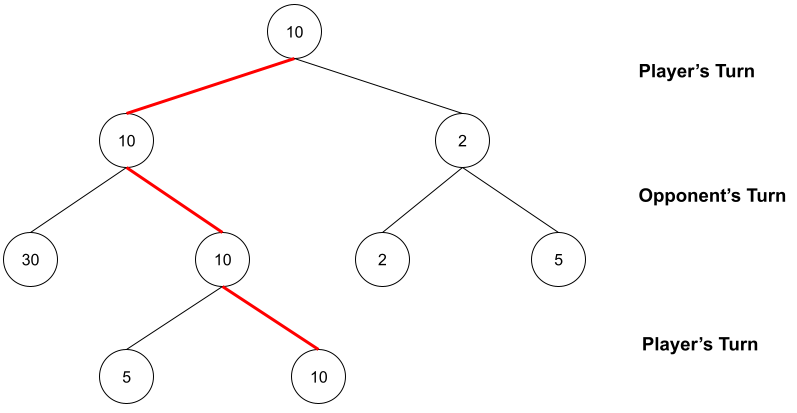
\includegraphics[width=\linewidth]{../img/Minimax1.png}
    \caption{Figure illustrating an exemplary game tree and decision based on minimax algorithm}
    \label{fig:minimax1}
\end{figure}

In Figure \ref{fig:minimax1}, consists of nodes that define either player's or the opponent's actions. For each action, there can be an evaluation where higher evaluation may mean it is favouring the player. For example, an action of the player causing two possible evaluations of 10 and 20 would mean the player would have higher advantage choosing the action leading to evaluation of 20. 

The minimax algorithm starts with a game tree with possible moves of the player and opponent. The evaluation of the leaf nodes positions are assigned, for example 5 and 10 in the figure. The player chooses a move to maximize the evaluation on their turn whereas the opponent wants to minimize the evaluation. The player chooses a move with an evaluation of 10 (between 10 and 5, maximizing its evaluation) and labels the action as 10. The player then determines that the opponent chooses an action that minimizes the evaluation, choosing an action with evaluation of 10 rather than 30. The player labels the parent node as 10 indicating that with best play, the player can achieve an evaluation of 10 from that node. The player then chooses the node with evaluation of 10 when choosing between 10 and 2, maximizing its evaluation and subsequently labels the parent node as 10. The red line shows the path the player determines as optimal leading to a decision choosing the the action labelled with evaluation of 10.

As the graph of a game can be large, one way to limit the search space for implementing the minimax algorithm is consider a depth-limited version of the algorithm. In this version, the algorithm only considers a part game tree with limited depth of the graph. Increasing the depth increases the accuracy of the decision at the cost of computational complexity. In terms of game, this depth may be equivalent to "looking ahead only a few moves".

In our implementation, the minimax algorithm is implemented with further optimizations including the alpha-beta pruning and the parallel version of the algorithm as described below:

\subsubsection{Alpha-beta pruning}

\begin{figure}[!ht]
    \centering
    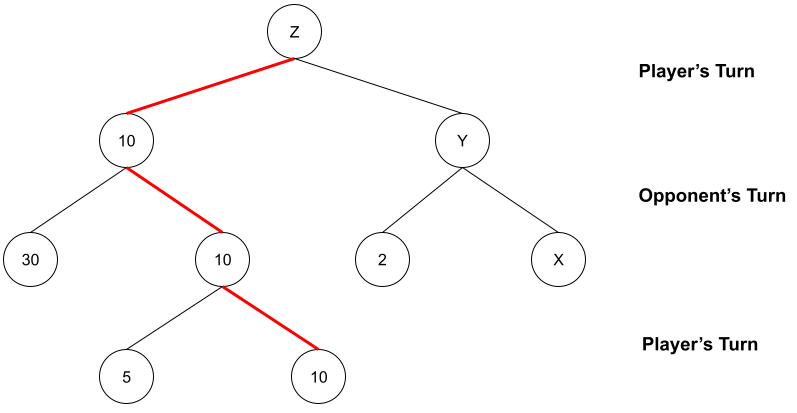
\includegraphics[width=\linewidth]{../img/Minimax2.png}
    \caption{Exemplary figure illustrating the alpha beta pruing for minimax algorithm}
    \label{fig:minimax2}
\end{figure}

In many cases, there may be the actions of the player in the search tree that can be evaluated worse than another action already evaluated. In such cases, where the better move or action has already been determined, it may not be useful to further evaluate the subsequent moves of the player and the opponent. Hence, the alpha-beta pruning reduces the game complexity by not further evaluating the branches of the node with evaluation worse than what has already been determined with another node.

As its name suggests, the alpha beta algorithm maintains two values, alpha and beta values. The alpha value stores the minimum score the player is assured to get while the beta value records the maximum score the opponent is assured to get. Whenever the evaluation of the minimum score of the player is higher than the maximum score after the subsequent move of the opponent (or in other words alpha > beta), the alpha-beta pruning algorithm stops evaluating the opponents position. This reduces the number of nodes in the search tree and hence reduces the complexity of the minimax algorithm.

In Figure \ref{fig:minimax2}, if the player determines that 
\begin{equation}
    Z = max (10, Y) = max (10,  min (2, X))
\end{equation}
, the value of X does not influence the value of $Y$ or $Z$ as $Y = min(2, X) \leq 2$ and hence $Z = max(10, \leq 2) = 10$. In this case, the player may not evaluate the branch $X$ or branch $Y$ further reducing the game tree and hence the computational complexity of the algorithm. 

Below, we list the implementation of the minimax algorithm with alpha beta pruning implementation:

\begin{lstlisting}
public TMove MinimaxStep(
    TGame game, int depth, bool maximizingPlayer, int alpha, int beta) {
    
    // return static evaluation if depth reached or game over
    // IStaticEvaluation

    bestMove = maximizingPlayer ? MinValue : MaxValue;
    
    // IValidMoves<TMove>
    foreach(var move in game.GetValidMoves())
    {
        // IMove<TMove>
        game.Move(move);

        //recursively call the MinimaxStep functino and update the
        //best score and move
        result = MinimaxStep(game, depth - 1, !maximizingPlayer);
        
        // IMove<TMove>
        game.UndoMove(move);

        if (maximizingPlayer)
        {
            if (result.Value > bestMove.Value)
            {
                bestMove.BestMove = move;
                bestMove.Value = result.Value;
            }
            if (bestMove.Value > beta)
                break;

            alpha = Math.Max(alpha, bestMove.Value);
        }
        else
        {
            if (result.Value < bestMove.Value)
            {
                bestMove.BestMove = move;
                bestMove.Value = result.Value;
            }
            if (bestMove.Value < alpha)
                break;

            beta = Math.Min(beta, bestMove.Value);
        }
    }
    return bestMove;
}
\end{lstlisting}

We have implemented a recursive minimax agent with alpha-beta pruning that is depth limited. The algorithm alternates with the variable \textit{maximizingPlayer} being 1 and 0 in each step indicating whether its the player's turn or the opponent's. In each case, the player determines the evaluation of the branch in the variable \textit{result} and sets the node as the best if it is the maximum (if player's turn) or minimum (if opponent's turn).

In the above implementation, the parameter depth is introduced to only consider the depth limited version of the algorithm, and alpha and beta variable limit the search space of the nodes in game tree.

\subsubsection{Parallel minimax}
Another way to improve the time complexity of the minimax algorithm is to parallelize the algorithm. The minimax algorithm involves in evaluating multiple nodes of the game tree. The way to parallelize such algorithm is to run different processes, in this case, evaluation of the position associated with different nodes, in different threads. This ensures that even though computational complexity may remain the same, the time complexity of the algorithm is distributed over multiple threads and possibly multiple processors.

The above defined methods to reduce the computational complexity of the minimax algorithm can be combined together. For example, the minimax algorithm can be depth limited and/or run with alpha-beta pruning and/or run in parallel as shown in the following implemented class.

\begin{lstlisting}
public class ParallelMinimaxABPruning<TPlayer, TMove, TGame>(int Depth) : IAIStrategy<TMove, TGame, TPlayer>
        where TGame : IMinimaxGame<TPlayer, TMove>, IDeepCopy<TGame>
    {
        private readonly object _lock = new();
        
        (*@{\hspace*{.5cm}\vdots}@*)
        
        private AIStrategyResult<TMove> ParallelMinimaxStep(TGame game, double alpha, double beta, int depth, bool maximizingPlayer)
        {
            (*@{\hspace*{.5cm}\vdots}@*)
            Parallel.ForEach(validMoves, (move, loopState) =>
            {
                var clonedGame = game.DeepCopy();
                clonedGame.Move(move);

                var result = ParallelMinimaxStep(clonedGame, alpha, beta, depth - 1, !maximizingPlayer);

                lock (_lock)
                {
                    if (maximizingPlayer)
                    {
                        (*@{\hspace*{.5cm}\vdots}@*)
                    }
                    else
                    {
                        (*@{\hspace*{.5cm}\vdots}@*)
                    }
                }
            });
            return bestMove;
        }
    }
\end{lstlisting}


\subsection{Monte-Carlo tree search agent}

\begin{figure}[!ht]
    \centering
    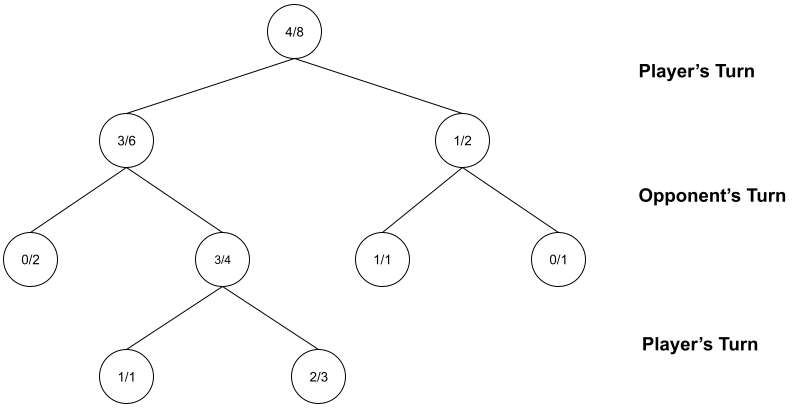
\includegraphics[width = \linewidth]{../img/MCTS1.png}
    \caption{Figure illustrating an iteration of the MCTS algorithm}
    \label{fig:MCTS1}
\end{figure}

\ac{MCTS} is a heuristic algorithm for searching the game tree based on Monte-Carlo simulations. As shown in Figure \ref{fig:MCTS1}, \gls{MCTS} algorithm determines the best path to the destination node in the game tree based on multiple trial runs through the game tree. In the figure, each node is labelled with a fraction where the denominator represents the total number of game runs through the node and the numerator represents the total number of wins for the player. For example, the game is simulated a total of 8 times in the example where the player wins 4 of the runs. The player wins 3/6 when taking an action while 1/2 when taking another action and so on.

The \gls{MCTS} algorithm builds upon the following framework:
\begin{enumerate}
    \item \textbf{Selection:} This step involves the algorithm choosing a move based on either a good move determined in previous iterations or a exploratory new move. In figure \ref{fig:MCTS1}, in the first player's turn, an action gives 3/6 chances of winning based on previous iterations whereas another gives 1/2 winning chances. The player selects a node that has highest possibility of winning, which in this case is equal. The player can also choose a new move that may be already explored to avoid not exploring further options.
    \item \textbf{Expansion:} This step involves the algorithm to add a new node to the game tree determined during the selection process. A node can simply be a valid move starting from the node from where no simulation step has been played out. In figure \ref{fig:MCTS2}, an unevaluated option (e.g., node inside the dotted box) is explored and simulated.
    \item \textbf{Simulation:} This step involves in playing out the game using policy. One of the policies can simply be a random policy (e.g., choosing a move based on certain distribution).
    \item \textbf{Back propagation:} Finally, based on the simulation step, this step involves in the algorithm updating the nodes. In figure \ref{fig:MCTS2}, the red arrows show the back propagation step as a result of exploration and simulation step where the probabilities or the weights of the nodes are updated as a result of exploration and simulation steps.
\end{enumerate}

\begin{figure}[!ht]
    \centering
    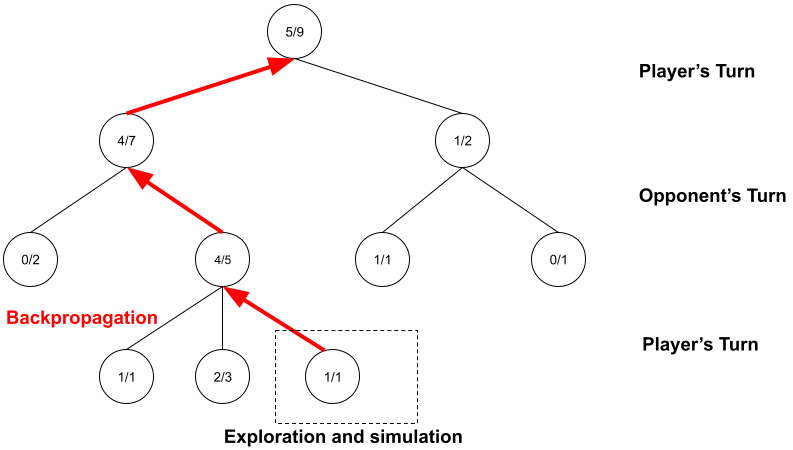
\includegraphics[width=\linewidth]{../img/MCTS2.png}
    \caption{Figure illustrating steps 2, 3, and 4 of the MCTS algorithm}
    \label{fig:MCTS2}
\end{figure}

The advantage of \gls{MCTS} algorithm over the minimax algorithm is that the \gls{MCTS} algorithm does not require any evaluation function as the weights are determined based on multiple simulation runs. On the contrary, the \gls{MCTS} algorithm requires multiple runs through the game to determine the weights.

\begin{lstlisting}
    public class MonteCarloTreeSearch<TMove, TGame, TPlayer> : IAIStrategy<TMove, TGame, TPlayer>
        where TGame : IMCTSGame<TGame, TMove, TPlayer>
        where TPlayer : IEquatable<TPlayer>
    {
    (*@{\hspace*{.5cm}\vdots}@*)    

        public AIStrategyResult<TMove> BestMove(TGame game, TPlayer player)
        {
            (*@{\hspace*{.5cm}\vdots}@*)
            for (int i = 0; i < _simulations; i++)
            {
                var selectedNode = Selection_Expansion(root);
                var winner = Simulation(selectedNode.State.DeepCopy());
                BackPropagation(selectedNode, winner);
            }
            (*@{\hspace*{.5cm}\vdots}@*)
        }

        private Node<TMove, TPlayer, TGame> Selection_Expansion(Node<TMove, TPlayer, TGame> node)
        {
            (*@{\hspace*{.5cm}\vdots}@*)
        }

        private TPlayer Simulation(TGame game)
        {
            (*@{\hspace*{.5cm}\vdots}@*)
        }

        private void BackPropagation(Node<TMove, TPlayer, TGame> node, TPlayer winner)
        {
            (*@{\hspace*{.5cm}\vdots}@*)        
        }
\end{lstlisting}

As described in the above code snippet, for \gls{MCTS} algorithm, the simulation is run \textit{${\_}simulations$} times and in each step, the game runs the four described steps. The best strategy is defined based on the Monte-Carlo runs and the determined final weights in the graph.

\subsection{A-Star agent}
A-Star is a search algorithm for traversing from the source node to the destination node while minimizing the cost function. The cost function, or "f" score, for a node depends on two components "g" value and "h" value. "g" value represents the distance from the source node to the node and "h" value represents the cost of the path from the node to the destination node, often defined by a heuristic. Mathematically,
\begin{equation}
    f = g + h
\end{equation}


\begin{lstlisting}

public class AStar<TMove, TMaze, TPlayer>
    where TPlayer : IAStarPlayer<TMove>
    where TMaze : INeighbors<TMove>
{
    public TMove BestMove(TMaze maze, TPlayer player)
    {
        (*@{\hspace*{.5cm}\vdots}@*)
        var openSet = new HashSet<Node<TMove>>() { start  };
        var closedSet = new HashSet<Node<TMove>>();
        (*@{\hspace*{.5cm}\vdots}@*)

        while (openSet.Count() > 0)
        {
            //get the node from the open set with the lowest f-score value
            var nodeWithLowestFscore = openSet.MinBy(s => s.FValue);
            currNode = nodeWithLowestFscore;

            //put this node in closed set and remove it from open set
            closedSet.Add(nodeWithLowestFscore);
            openSet.Remove(nodeWithLowestFscore);

            (*@{\hspace*{.5cm}\vdots}@*)
            
            //INeighbors<TMove>
            foreach (var neighbor in maze.Neighbors(currNode.CurrMove))
            {
            (*@{\hspace*{.5cm}\vdots}@*)
            if (!openSet.Contains(neighborNode) || neighborNode.GValue < gScore)
                {
                    neighborNode.GValue = gScore;
                    neighborNode.HValue = player.CalculateHeuristic(neighbor);
                    neighborNode.FValue = gScore + neighborNode.HValue;
                    (*@{\hspace*{.5cm}\vdots}@*)
                }
            }
        }
        (*@{\hspace*{.5cm}\vdots}@*)
    }

\end{lstlisting}

The A-star algorithm starts by maintaining two sets \textit{openSet} and \textit{closedSet}. \textit{openSet} consists of nodes with children not yet visited and \textit{closedSet} consists of nodes with children nodes explored already. The node with lowest cost function ("f" score) is explored and marked as the \textit{currentNode} from the \textit{openSet}. Subsequently, the 'f' scores of the neighbours of the \textit{currentNode} is calculated. This algorithm runs until the destination node in the tree is reached.

\section{Generalization of AI interface to other games}
\label{TicTacToe}

In this section, we demonstrate how seamless it is to integrate the \gls{AI} agents with our implementation to other games. We will use an example to integrate our interface to the tic-tac-toe game for this purpose.

The interfaces with our implementation as described earlier  are parametrized over 3 generic types, namely TGame, TMove and TPlayer. For Tic-tac-toe, we will use the \textit{int} type for TMove and TPlayer parameteters. For TGame, we will use the \textbf{TicTacToe} class type.

\begin{lstlisting}
public class TicTacToe :
    ITerminal, //Minimax, MCTS
    IValidMoves<int>, //Minimax, MCTS
    IMove<int>, //Minimax, MCTS
    IPlayer<int>, //Minimax, MCTS
    IOpponent<int>, //MCTS
    IDeepCopy<TicTacToe>, //MCTS
    IWinner<int>, //MCTS
    IStaticEvaluation //Minimax
\end{lstlisting}

For the Tic-Tac-Toe game, we will need a 3x3 array representing the game board, and a property turn that represents which player's turn it currently is. Turn therefore will have 2 values, 1 and 2 representing player 1 and player 2 respectively.

\begin{lstlisting}
private int[,] Cells = new int[3, 3];
private int turn = 1; // 1 -> p1, 2 -> p2
\end{lstlisting}

The game board, represented by \texttt{Cells} property, is initially all zeros. Over the course of the game, it will contain values 0, 1 or 2.

We will now implement all the interfaces above. We start by implementing the \textbf{IValidMoves\textless{}int\textgreater{}} iterface. To get all the valid locations, i.e Cells marked by 0, we can encode the Cell's i and j position by the following equation
\begin{equation}
\label{eq:Move}
    Move(C_{ij}) = i + 3 * j
\end{equation}

As an example, consider the cell $C_{1,2}$. From equation \ref{eq:Move}, we have that $Move(C_{1,2}) = 1 + 3 * 2 = 7$.

\begin{lstlisting}
public IEnumerable<int> GetValidMoves() {
    for(int i =  0; i < 3; i++)
        for (int j = 0; j < 3; j++)
            if (Cells[i, j] == 0)
                yield return i + 3 * j;
}
\end{lstlisting}

We now write a method \textit{Place} that takes in two arguments, move and mark, move being an integral value repesented by equation \ref{eq:Move}, and mark being one of 0, 1, 2. 1 and 2.
On each placement, we can also retrieve the winner(if any) and get information on whether the game terminated, so we implement both the \textbf{ITerminal.HasFinished} and \textbf{IWinner.Winner} properties. To check if the game has finished we check if 3 adjacent sides of the game board are filled by the same player. These include diagonals too.
We define \textbf{Winner} to hold 4 possible values - 1 and 2 indicating player 1 and player 2 victory respectively, 0 indicating a draw and -1 indicating that the game is still in progress.
Before all these, we firstly need to decompose the move we encoded by equation \ref{eq:Move} to i and j values. To do so from given move $Move(C_{ij})$, we can use the following equations:
\begin{equation}
    i = Move(C_{ij}) \mod 3
\end{equation}
\begin{equation}
    j = \frac{Move(C_{ij})}{3}
\end{equation}
We then place one of 'X' or 'O' signs, (or remove them if we want to undo the last action), check if any player won, and if not, switch turns.

\begin{lstlisting}
public bool HasFinished => CheckWin();

// 0 draw, 1 -> p1, 2 -> p2, -1 game in progress
private int _winner = -1; 

public int Winner => _winner;

private void Place(int move, int item) {
    int i = move % 3;
    int j = move / 3;
    Cells[i, j] = item;
    CheckWin();
    turn = turn % 2 + 1;
}

void CheckWin() {
    //check all 3 consecutive adjecent squares (including
    //diagonals), and return true if they're filled by the
    //same player.
    // update the _winner variable based on this
}

\end{lstlisting}

We can then implement the \texttt{Move} and \texttt{UndoMove} methods. Both these methods use the \texttt{Place} method.
We also switch turns after a successful Move/UndoMove operation.
\begin{lstlisting}
 public void Move(int move) {
    Place(move, turn);
}

public void UndoMove(int move) {
    Place(move, 0);
}
\end{lstlisting}

We also need to implement the \texttt{CurrentPlayer} and \texttt{Opponent} properties implemented by the \textbf{IPlayer} and \textbf{IOpponent} interfaces respectively. We simply use the value held by the \textbf{turn} variable in our implementation to return it. The \textbf{turn} variable holds the index of the current player, so for the opponent, we simply return the value not held by the \textbf{turn} variable.

\begin{lstlisting}
public int CurrentPlayer => turn;

public int Opponent => turn % 2 + 1;    
\end{lstlisting}

To have the Tic-Tac-Toe implementation work smoothly with the Minimax algorithm, we also implement the \textbf{IStaticEvaluation.Evaluate()} method.
\begin{lstlisting}
public double Evaluate ( bool currentMaximizer ) {
    if ( _winner == CurrentPlayer ) return 1.0;
    if ( _winner == Opponent ) return -1.0;
    return 0.0;
}
\end{lstlisting}

Finally, we implement the \textbf{IDeepCopy} interface. This interface is used by the \gls{MCTS} algorithm, especially during the simulation phase so as to not change the original game state or properties references in any way possible.

\begin{lstlisting}
public TicTacToe DeepCopy() {
    var t = new TicTacToe();
    //shallow copy of struct(int in our case) is
    //fine since no reference is copied
    t.Cells = (int[,])Cells.Clone();
    t.turn = turn;
    return t;
}
\end{lstlisting}

We can now use the Minimax, Monte Carlo Tree Search, Minimax Alpha-beta pruning, Parallel Minimax Alpha-beta pruning, Random agents to play the game of tic-tac-toe. For example:

\begin{lstlisting}
var tt = new TicTacToe();

//MinimaxABPruning<TPlayer, TMove, TGame>
var minimaxABagent = new MinimaxABPruning<int, int, TicTacToe>(...);

//MonteCarloTreeSearch<TMove, TGame, TPlayer>
var mctsAgent = new MonteCarloTreeSearch<int, TicTacToe, int>(...);

minimaxBestMove = minimaxABAgent.BestMove(tt, tt.turn).BestMove;
tt.Move(minimaxBestMove);

mctsBestMove(tt, tt.turn).BestMove;
tt.Move(mctsBestMove);
\end{lstlisting}

This way, we can play the Tic-Tac-Toe game between 2 smart or trivial agents until the game finishes.

\section{Quoridor Game Implementation}

\begin{figure}[!ht]
    \centering
    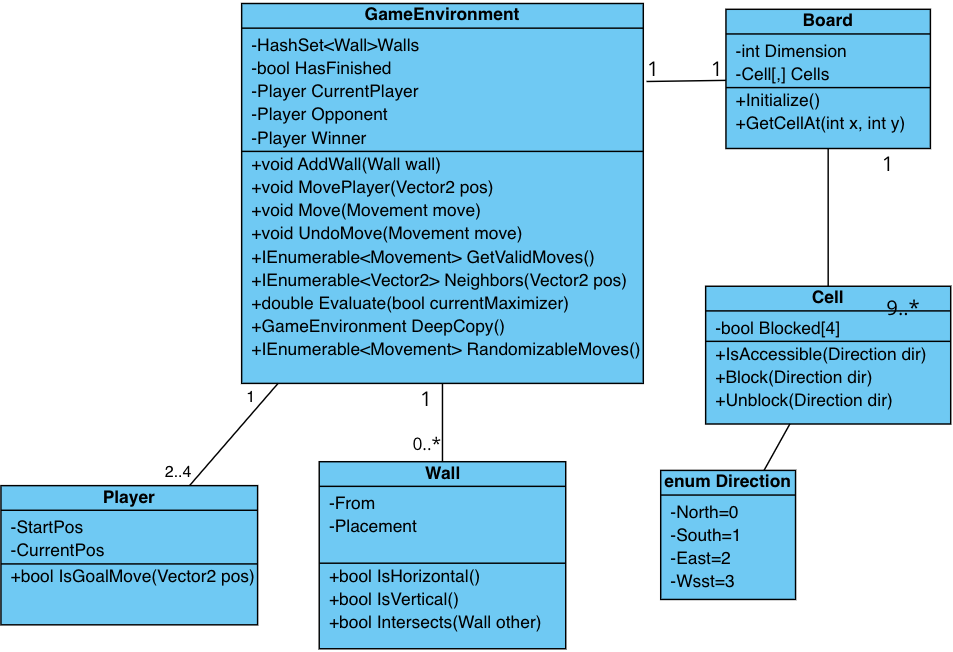
\includegraphics[width=.95\linewidth]{../img/uml_core.png}
    \caption{A UML diagram depicting relationship in the core library}
    \label{fig:core_uml}
\end{figure}

As seen in figure \ref{fig:core_uml}, the \texttt{GameEnvironment} class implements all interfaces necessary for \gls{AI} integration.
In contrast to the \textbf{Tic-Tac-Toe} implementation we saw earlier in section \ref{TicTacToe} where \texttt{int} type was used for the \texttt{TMove} parameter, we use a reference type \texttt{Movement} for the \texttt{TMove} parameter, since we need to consider wall placement, player movement, which is very difficult to encode and decode as integral values.
\begin{lstlisting}
public abstract class Movement{}

public class Vector2 : Movement{...}

public class Wall : Movement{...};
\end{lstlisting}
This approach makes it easier to identify movement types and therefore easily perform Move/Unmove operations on the game and much more.

We will now describe the core elements of the interfaces that we integrated for this game.

\begin{lstlisting}
public IEnumerable<Movement> GetValidMoves() {
    List<Vector2> neighborMoves;
    //Populate the moves based on whether the neighboring
    //cells are accessible from the cell the current player
    //is in

    List<Wall> possibleWalls;
    //Populate the available wall list. We don't include
    //already placed walls/walls intersecting with already
    //placed walls

    return neighborMoves.Concat(possibleWalls);
}
\end{lstlisting}

Also, as described earlier, for the move and unmove operations, we do not need to decipher the movement by a pre-defined rule like we did in section \ref{TicTacToe}. We can easily check the underlying type of the abstract Movement type and do operations accordingly.

\begin{lstlisting}
public void Move(Movement move) {
    if (move is Vector2 v2) {
        MovePlayer(v2);
    }
    if (move is Wall wall) {
        AddWall(wall);
    }
    //change turn
}
\end{lstlisting}

As for the static evaluation function required by the Minimax algorithm, we use the following features of the game:
\begin{itemize}
    \item 
\end{itemize}

\subsection{Project Structure}

The solution consists of six fundamental projects, each written in \gls{Csharp}.

\begin{itemize}
    \item \textbf{Quoridor.Core}\\
        This library project contains the core game logic for Quoridor, and implements all interfaces to allow \gls{AI} algorithms to run.
        
    \item \textbf{Quoridor.AI}\\
        This library project includes all the fundamental interfaces and a generic \gls{AI} algorithms implemented using these interfaces.

    \item \textbf{Quoridor.Common}\\
        This library project includes all common helpers, such as XML parser helper, logging helper, etc.

    \item \textbf{Quoridor.Tests}\\
        This NUnit test project includes all unit tests for robust development.

    \item \textbf{Quoridor.ConsoleApp}\\
        A CLI tool that runs simulations and allows user to play against an opponent with a visual interface.

    \item \textbf{Quoridor.DesktopApp}\\
        A WinForms application that allows user to play against one another or against various \gls{AI}.
\end{itemize}

These projects are inter-connected by references. For example from figure \ref{fig:proj_dep}, \textbf{Quoridor.AI} is a standalone library that contains all the interfaces, which is referenced by all other projects.
All project dependency structures are depicted in figure \ref{fig:proj_dep}.

\begin{figure}[!ht]
    \centering
    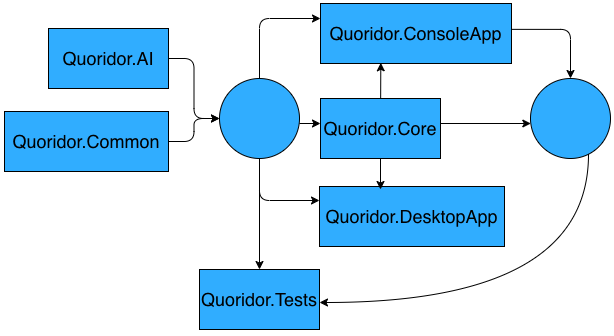
\includegraphics[width=.95\linewidth]{../img/project_structure.png}
    \caption{Quoridor project dependency diagram}
    \label{fig:proj_dep}
\end{figure}